\documentclass[10pt]{book}
\usepackage[utf8]{inputenc}
\usepackage[italian]{babel}
\usepackage{multicol}
\usepackage[bookmarks]{hyperref}
\usepackage[a4paper, total={18cm, 25cm}]{geometry}
\usepackage{listings}
\usepackage{graphicx}
\usepackage{makecell}
\graphicspath{ {./img/} }
\usepackage{color}
\definecolor{mygray}{rgb}{0.5,0.5,0.5}
\usepackage{listings}
\lstset{
	language=SQL,
	breaklines=true,
	keywordstyle=\bfseries,
	identifierstyle=\ttfamily,
	commentstyle=\color{mygray},
	morekeywords={database, REFERENCES, SCHEMA, AUTHORIZATION, PROCEDURE},
}

\begin{document}
\renewcommand*\contentsname{Indice}
\title{Basi di Dati}
\author{Federico Matteoni}
\date{A.A. 2019/20}
\maketitle
\tableofcontents
\pagebreak
\chapter*{Introduzione}
\paragraph{Obiettivi del corso} Modelli dei dati, linguaggi e sistemi per lo sviluppo di applicazioni che prevedono l'uso di grandi quantità di dati permanenti organizzati in \textbf{basi di dati}.
\paragraph{Testo di Riferimento} \textit{Fondamenti di Basi di Dati}, A. Albano, G. Ghelli e R. Orsini, Zanichelli. Scaricabile liberamente da \texttt{fondamentidibasididati.it}
\paragraph{Terminologia}
\begin{list}{}{}
	\item \textbf{Base di dati}: tecnologia di base, gestione delle attività quotidiane dell'organizzazione e \textbf{tema di questo corso}
	\item Data Warehouse, Data Lake, Big Data, Data Science: termini che hanno a che vedere con l'\textbf{analisi dei dati} e che non rientrano nei temi trattati nel corso.
\end{list}
\chapter{Costruzione di una base di dati}
\paragraph{Cos'è una base di dati?} Una \textbf{base di dati} è un \textbf{insieme organizzato di dati} usati per il supporto allo svolgimento di un'attività (di un ente, azienda, ufficio, persona\ldots)
\paragraph{Qualche esempio}
\begin{center}
\textbf{Materie}\\
	\begin{tabular}{c | c | c}
	\textbf{Titolo} & \textbf{Codice} & \textbf{Syllabus} \\
	\hline
	Basi di Dati & AA024 & Progettazione e interrogazione\ldots \\
	\hline
	Reti di Calcolatori & AA019 & Realizzazione e uso di reti, protocollo TCP\ldots
	\end{tabular}
\end{center}
\begin{center}
\textbf{Corsi}\\
	\begin{tabular}{c | c | c | c}
	\textbf{Materia} & \textbf{AA} & \textbf{Semestre} & \textbf{Titolare} \\
	\hline
	AA024 & 2007 & 1 & Albano \\
	\hline
	AA024 & 2007 & 1 & Ghelli \\
	\hline
	AA019 & 2007 & 1 & Brogi 
	\end{tabular}
\end{center}
\section{Elementi}
\subsection{Figure Coinvolte}
\begin{list}{}{}
	\item \textbf{Committente}
	\begin{list}{}{}
		\item Dirigente
		\item Operatore
	\end{list}
	\item \textbf{Fornitore}
	\begin{list}{}{}
		\item Direttore del progetto
		\item Analista
		\item Progettista del DB
		\item Programmatore di applicazioni che usano il DB
	\end{list}
	\item Manutenzione e messa a punto del DB -- \textbf{Gestione del DBMS}
	\begin{list}{}{}
		\item Amministratore del DBMS
	\end{list}
\end{list}
\subsection{Sistemi Informativi}
\paragraph{Definizione} Un \textbf{sistema informativo} di un'organizzazione è una \textbf{combinazione di risorse, umane e materiali, e di procedure} organizzate per raccolta, archiviazione, elaborazione e scambio \textbf{delle informazioni} necessarie alle attività:
\begin{list}{}{}
	\item \textbf{Operative} (informazioni di servizio)
	\item Programmazione e \textbf{controllo} (informazioni di gestione)
	\item \textbf{Pianificazione} strategica (informazioni di governo)
\end{list}
\pagebreak
\paragraph{Esempi di sistemi informativi}
\begin{list}{}{Un comune}
	\item Gestione servizi demografici (anagrafe, stato civile, servizio elettorale e vaccinale) e della rete viaria
	\item Gestione attività finanziaria secondo la normativa vigente
	\item Gestione del personale per il calcolo della retribuzione in base al tipo di normativa contrattuale
	\item Gestione dei servizi amministrativi e sanitari delle USL
	\item Gestione della cartografia generale e tematica del territorio
\end{list}
\paragraph{Sistema informativo nelle organizzazioni}
\begin{center}
	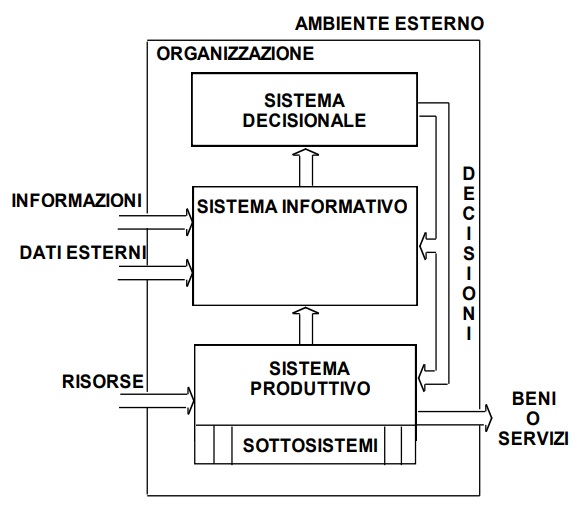
\includegraphics[scale=0.7]{sisinformativoorg.png}
\end{center}
\subsection{Sistemi Informatici}
\paragraph{Sistema Informativo Automatizzato} Quella parte del sistema informativo in cui le informazioni sono raccolte, elaborate, archiviate e scambiate usando un \textbf{sistema informatico}.
\paragraph{Sistema Informatico} Insieme delle tecnologie informatiche e della comunicazione (\textbf{ICT}, Information and Communication Technologies) a supporto delle attività di un'organizzazione.
\paragraph{Terminologia}
\begin{center}
Sistema informativo $\longrightarrow$ Sistema informativo automatizzato\\
Sistema informativo automatizzato $\longrightarrow$ Sistema informatico
\end{center}
\begin{center}
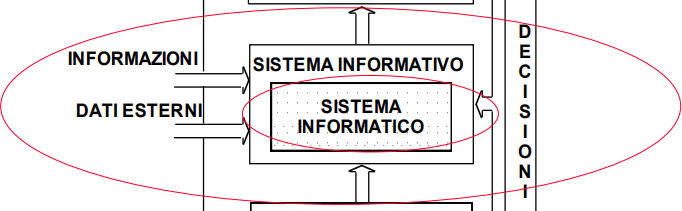
\includegraphics[scale=0.7]{sisinformativoorg2.png}
\end{center}
\pagebreak
\subsection{Classificazione dei sistemi informatici}
\begin{center}
Sistemi Informatici Operativi $\longrightarrow$ Sistemi Informatici Direzionali
\end{center}
\begin{multicols}{2}
\paragraph{Sistemi Informatici Operativi} I dati sono organizzati di DB. Le applicazioni si usano per svolgere le classiche attività strutturate e ripetitive dell'azione nelle aree amministrativa e finanziaria: vendite, risorse umane, produzione\ldots\\
\textbf{Alcune sigle}:
\begin{list}{}{}
	\item \textbf{DP} Data Processing\\\textbf{EDP} Electronic Data Processing
	\item \textbf{TPS} Transaction Processing Systems
\end{list}
\begin{center}
	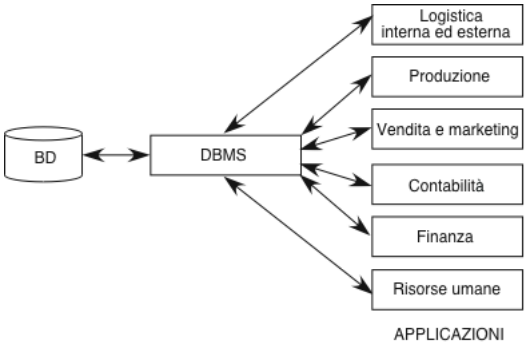
\includegraphics[scale=0.6]{sisinfop.png}
\end{center}
\paragraph{DBMS} Le caratteristiche del DB sono \textbf{garantite da un sistema per la gestione della base di dati} (\textbf{DBMS}, Data Base Management System) che ha il controllo dei dati e li rende accessibili agli utenti autorizzati.
\paragraph{OLTP} \textbf{On-Line Transaction Processing}, modo d'uso principale dei DBMS. Tradizionale elaborazione di transazioni, che realizzano processi operativi per il funzionamento di organizzazioni:
\begin{list}{}{}
	\item Operazioni predefinite e relativamente semplici
	\item Ogni operazione coinvolge \textit{pochi} dati
	\item Dati di dettaglio, aggiornati
\end{list}
\end{multicols}
\begin{multicols}{2}
\paragraph{Sistemi Informatici Direzionali} I dati sono organizzati in data warehouse (DW) e gestiti ad un opportuno sistema. Le applicazioni, dette di \textbf{business intelligence}, sono strumenti di supporto ai processi di controllo delle prestazioni aziendali e di decisione manageriale. Terminologia:
\begin{list}{}{}
	\item \textbf{MIS} Management Information Systems
	\item \textbf{DSS} Decision Support Systems, data-based o model-based
	\item \textbf{EIS} Executive Information System
\end{list}
\begin{center}
	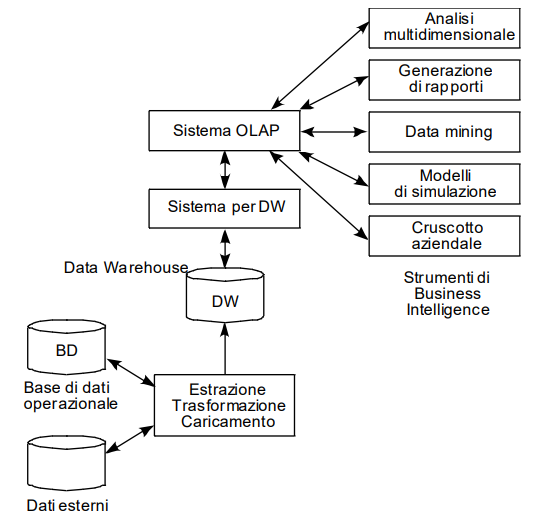
\includegraphics[scale=0.6]{sisinfdir.png}
\end{center}
\columnbreak
\paragraph{OLAP} \textbf{On-Line Analytical Processing} modo d'uso principale dei DW. Analisi dei dati di supporto alle decisioni:
\begin{list}{}{}
	\item Operazioni complesse e casuali
	\item Ogni operazione può coinvolgere \textit{molti} dati
	\item Dati aggregati, storici, anche non attualissimi
\end{list}
\end{multicols}
\pagebreak
\paragraph{Differenze tra OLTP e OLAP}
\begin{center}
	\begin{tabular}{r | l | l}
	 & \makecell{\textbf{OLTP}} & \makecell{\textbf{OLAP}} \\
	\textbf{Scopi} & Supporto operatività & Supporto decisioni \\
	\textbf{Utenti} & Molti, esecutivi & Pochi, dirigenti e analisti \\
	\textbf{Dati} & Analitici, relazionali & Sintetici, multidimensionali \\
	\textbf{Usi} & Noti a priori & Poco prevedibili \\
	\textbf{Quantità di dati per attività} & Bassa (decine) & Alta (milioni) \\
	\textbf{Orientamento} & Applicazione & Soggetto \\
	\textbf{Aggiornamenti} & Frequenti & Rari \\
	\textbf{Visione dei dati} & Corrente & Storica \\
	\textbf{Ottimizzati per} & Transazioni & Analisi
	\end{tabular}
\end{center}
\subsection{Requisiti per l'Analisi dei Dati}
\paragraph{Aggregati} Non interessa \textbf{un} dato, ma la \textbf{somma}, la \textbf{media}, il \textbf{minimo}/\textbf{massimo} di una misura\ldots
\paragraph{Multidimensionale} Interessa \textbf{incrociare le informazioni}, per analizzarle da punti di vista diversi e valutare i risultati del business per intervenire sui problemi critici o per cogliere nuove opportunità
\paragraph{Diversi livelli di dettaglio} Per esempio, una volta scoperto un calo delle vendite in un determinato periodo in una specifica regione, si passa ad un'analisi dettagliata nell'area di interesse per cercare di scoprirne le cause (dimensioni con \textbf{gerarchie})
\subsection{Big Data}
\paragraph{Ampio} Big data è un termine ampio riferito a situazioni in cui l'approccio "schema-first" tipico di DB e DW risulta troppo restrittivo o troppo lento.
\paragraph{3 V} Volume, Varietà, Velocità
\paragraph{} I Big Data sono in genere associati a sistemi NoSQL, machine learning e approcci Data Lake.
\section{DBMS}
Un \textbf{DBMS} è un sistema (\textbf{software}) in grado di \textbf{gestire collezioni di dati} che siano, tra le altre cose:
\begin{list}{}{}
	\item \textbf{Grandi}
	\item \textbf{Persistenti}, con un periodo di vita indipendente dalle singole esecuzioni dei programmi che le utilizzano
	\item \textbf{Condivise}, usate da applicazioni diverse
\end{list}
garantendo \textbf{affidabilità} (resistenza a malfunzionamenti hardware e software-recovery) e \textbf{privacy} (con una disciplina e un controllo degli accessi).\\
Come ogni altro software, un DBMS deve essere \textbf{efficiente} (usare al meglio le risorse di spazio e tempo del sistema) ed \textbf{efficace} (rendere produttive le attività degli utilizzatori).\\
Un DBMS offre opportuni linguaggi per:
\begin{list}{}{}
	\item \textbf{Definire lo schema} di un DB, che va definito prima di creare dati
	\item \textbf{Scegliere le strutture dati} per la memorizzazione
	\item Memorizzare i dati \textbf{rispettando i vincoli} definiti nello schema
	\item Recuperare e modificare i dati, interattivamente (\textbf{query language}, linguaggio di interrogazione) o da programmi
\end{list}
\subsection{Dati}
I dati permanenti contenuti in un DB sono divisi in due categorie:
\begin{list}{}{}
	\item \textbf{Metadati}\\
	Descrivono datti sullo schema dei dati, utenti autorizzati, applicazioni, parametri quantitativi\ldots\\
	I metadati sono descritti da uno schema usando il modello dei dati usato dal DBMS e sono interrogabili con le stesse modalità previste dai dati
	\item \textbf{Dati}\\
	Rappresentazioni di certi fatti conformi alle definizioni dello schema. Hanno le seguenti caratteristiche:
	\begin{list}{}{}
		\item Organizzati in \textbf{insiemi strutturati e omogenei}, fra i quali sono definite delle \textbf{relazioni}. La struttura dei dati e le relazioni sono \textbf{descritte nello schema} usando i meccanismi di astrazione del modello dei dati del DBMS.
		\item Sono \textbf{molti}, sia in assoluto che rispetto ai metadati, e non possono essere gestiti in memoria temporanea
		\item Sono \textbf{accessibili mediante transazioni}, \textbf{unità di lavoro atomiche} che \textbf{non possono avere effetti parziali}
		\item Sono \textbf{protetti} sia \textbf{da accesso da parte di utenti non autorizzati}, sia \textbf{da corruzione dovuta a malfunzionamenti} hardware o software
		\item Sono \textbf{utilizzabili contemporaneamente da utenti diversi}
	\end{list}
\end{list}
Il \textbf{modello relazionale dei dati} è il più diffuso fra i DBMS commerciali. Il \textbf{meccanismo di astrazione} fondamentale è la \textbf{relazione} (\textbf{tabella}), sostanzialmente un insieme di record dai campi elementari.\\
Lo schema di una relazione ne definisce il nome e ne descrive la struttura dei possibili elementi della relazione (insieme di attributi con il loro tipo)
\paragraph{Esempio}
\begin{list}{}{}
	\item \textbf{Definizione del DB}
	\begin{lstlisting}
create database EsempioEsame
	\end{lstlisting}
	\item \textbf{Definizione schema}
	\begin{lstlisting}
create table Esami(Materia char(5), Candidato char(8), Voto int, Lode char(1),
Data char(6))
	\end{lstlisting}
	\item \textbf{Inserzione dati}
	\begin{lstlisting}
insert into Esami values ('BDSI1', '080709', 30 'S', '070900')
	\end{lstlisting}
	\item \textbf{Interrogazione}
	\begin{lstlisting}
select Candidato from Esami where Materia = "BDSI1" and Voto = 30
	> Candidato
	> 080709
	\end{lstlisting}
\end{list}
\pagebreak
\subsection{DDL}
\paragraph{Data Definition Language} Linguaggio per la definizione della base di dati.\\
Utile distinguere tre diversi livelli di descrizione dei dati (\textbf{schemi}):
\begin{multicols}{2}
\begin{list}{}{}
	\item Livello di \textbf{vista logica}
	\item Livello \textbf{logico}
	\item Livello \textbf{fisico}
\end{list}
\begin{center}
	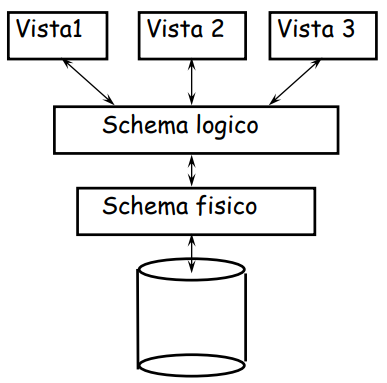
\includegraphics[scale=0.5]{livellidescrdati.png}
\end{center}
\end{multicols}
\paragraph{Livello Logico} Descrive la struttura degli insiemi di dati e delle relazioni fra loro, secondo un erto modello dei dati, senza nessun riferimento alla loro organizzazione fisica nella memoria permanente.\\
Esempi:
\begin{lstlisting}
Studenti(Matricola char(8), Nome char(20), Login char(8), Anno int, Reddito float)
Corsi(IdeC char(8), Titolo char(20), Credito int)
Esami(Matricola char(8), IdeC char(8), Voto int)
\end{lstlisting}
\paragraph{Livello Fisico} Descrive come vanno organizzati fisicamente i dati nelle memorie permanenti e quali strutture dati ausiliarie prevedere per facilitarne l'uso (schema fisico o interno).\\
Esempi: relazioni Studenti e Esami organizzate in modo seriale, Corsi organizzata sequenziale con indice, indice su Matricola.
\paragraph{Vista Logica} Descrive come deve \textbf{apparire la struttura} del DB ad una certa applicazione (\textbf{schema esterno} o \textbf{vista}). Esempio:
\begin{lstlisting}
InfCorsi (IdeC char(8), Titolo char(20), NumEsami int)
\end{lstlisting}
Nell'organizzazione di una banca, lo \textbf{schema logico} conterrà tutte le tabelle e i dati relativi ai conti correnti, ma anche al personale. Lo schema logico conserva \textbf{tutte le informazioni} della banca. Nello \textbf{schema esterno} ogni correntista potrà \textbf{accedere solo ad alcune informazioni} di suo interesse: quelle del proprio conto corrente.
\paragraph{Indipendenza} L'approccio con tre livelli è stato proposto per garantire le proprietà di indipendenza logica e fisica dei dati, fra gli obiettivi più importanti dei DBMS.
\begin{list}{}{}
	\item \textbf{Indipendenza fisica}: i programmi applicativi non devono essere modificati in seguito a modifiche dell'organizzazione fisica dei dati
	\item \textbf{Indipendenza logica}: i programmi applicativi non devono essere modificati in seguito a modifiche dello schema logico
\end{list}
\subsection{DML}
\paragraph{Data Manipulation Language} Linguaggio per l'uso dei dati.\\
Un DBMS deve prevedere più modalità d'uso per soddisfare esigenze di diverse categorie d'utenti: GUI per accedere ai dati, linguaggio di interrogazione per i non programmatori, linguaggio di programmazione per chi sviluppa le applicazioni, linguaggio di sviluppo per le interfacce delle applicazioni.\\
Linguaggi vari e interfacce diverse:
\begin{list}{}{}
	\item Linguaggi testuali interattivi, SQL
	\item Comandi (come quelli del linguaggi interattivo) immersi in un linguaggio ospite, come il C
	\item Comandi (come quelli del linguaggi interattivo) immersi in un linguaggio ad hoc (come PL/SQL) con anche altre funzionalità (come grafici e stampe strutturate)
	\item Interfacce amichevoli
\end{list}
\subsection{Schemi e Istanze}
\paragraph{Schema} Descrive la \textbf{struttura dei dati}, sostanzialmente invariante nel tempo: le "classi", intestazione delle tabelle
\paragraph{Istanza} \textbf{Valori attuali} dei dati che possono cambiare anche molto rapidamente: gli "oggetti", il corpo di ciascuna tabella
\subsection{Meccanismi per il controllo dei dati}
Caratteristica molto importante dei DBMS è il tipo di meccanismi usati per garantire le seguenti proprietà
\begin{list}{}{}
	\item \textbf{Integrità}: mantenimento delle proprietà specificate nello schema
	\item \textbf{Sicurezza}: protezione da usi non autorizzati
	\item \textbf{Affidabilità}: protezione da malfunzionamenti e interferenze dovute all'accesso concorrente di più utenti
\end{list}
\subsection{Transazioni}
\paragraph{Definizione} Una \textbf{transazione} è una \textbf{sequenza di azioni di lettura/scrittura in memoria permanente e di elaborazione dati in memoria temporanea}, con le seguenti proprietà:
\begin{list}{}{}
	\item \textbf{Atomicità}: le transazioni che terminano prematuramente (\textbf{aborted transactions}) sono \textbf{trattate dal sistema come se non fossero mai iniziate}. Eventuali effetti sul DB sono \textbf{annullati}.
	\item \textbf{Serializzabilità}: esecuzioni concorrenti di più transazioni danno come effetto quello di una esecuzione seriale
	\item \textbf{Persistenza}: le \textbf{modifiche} sul DB di una transazione terminata normalmente sono \textbf{permanenti}, cioè \textbf{non alterabili da malfunzionamenti}
\end{list}
\section{Progettazione}
\paragraph{Progettare} Progettare un DB significa \textbf{progettare la struttura dei dati e delle applicazioni}. La progettazione dei dati è l'attività più importante e per progettare al meglio i dati è necessario che essi siano un \textbf{modello fedele del dominio} in esame. Per questo ora parleremo della \textbf{modellazione}.
\subsection{Modellazione}
\paragraph{Definizione} Un \textbf{modello astratto} è la \textbf{rappresentazione formale di idee e conoscenze relative ad un fenomeno}.\\
Aspetti di un modello:
\begin{list}{}{}
	\item Il \textbf{modello} è la \textbf{rappresentazione di certi fatti}.
	\item La \textbf{rappresentazione} è \textbf{data con un linguaggio formale}.
	\item Il \textbf{modello} è \textbf{il risultato di un processo di interpretazione}, guidato dalle idee e conoscenze possedute dal soggetto che interpreta.
\end{list}
\textbf{La stessa realtà può utilmente essere modellata in modi diversi e a diversi livelli di astrazione}.
\begin{center}
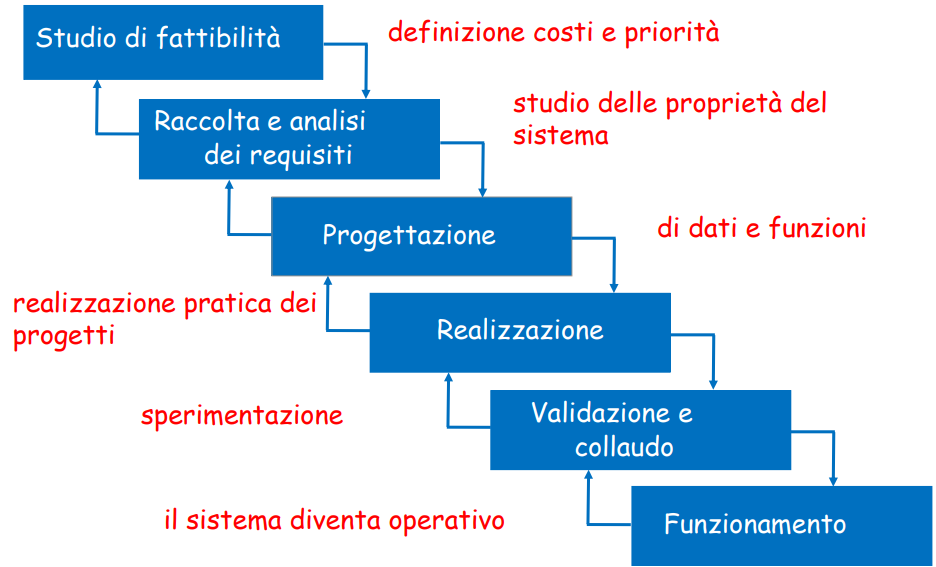
\includegraphics[scale=0.7]{modellaz.png}
\end{center}
\paragraph{Metodologia di progetto} Per garantire prodotti di buona qualità è opportuno seguire una metodologia di progetto, con:
\begin{list}{}{}
	\item Articolazione delle attività in fasi (\textbf{decomposizione})
	\item Criteri di scelta (\textbf{strategie})
	\item \textbf{Modelli} da rappresentare
	\item \textbf{Generalità} rispetto al problema in esame e agli strumenti a disposizione
	\item \textbf{Qualità} del prodotto
	\item \textbf{Facilità d'uso}
\end{list}
\paragraph{Progettazione della base di dati} Suddivisa nelle seguenti fasi:
\begin{enumerate}
	\item \textbf{Analisi} dei requisiti
	\item Progettazione \textbf{concettuale}
	\item Progettazione \textbf{logica}
	\item Progettazione \textbf{fisica}
\end{enumerate}
Ciascuna fase è incentrata sulla modellazione, che discuteremo quindi con riferimento alla problematica della progettazione del DB.
\paragraph{Modello dei dati} Insieme di costrutti utilizzati per organizzare i dati di interesse e descriverne la dinamica. Il componente fondamentale è l'insieme dei \textbf{meccanismi di strutturazione} (o \textbf{costruttori di tipo}). Come nei linguaggi di programmazione, esistono meccanismi che permettono di definire nuovi tipi, così \textbf{ogni modello dei dati prevede alcuni costruttori}: per esempio, il \textbf{modello relazionale prevede il costruttore \textit{relazione}}, che permette di definire insiemi di record omogenei.
\pagebreak
\subsection{Aspetti del problema}
\subsubsection{Aspetto ontologico} Quale conoscenza del dominio del discorso si rappresenta? Ontologico cioè studio di ciò che si suppone esista nell'universo del discorso e che sia quindi necessario modellare.
\begin{list}{}{Cosa si modella:}
	\item \textbf{Conoscenza concreta}: i fatti
	\item \textbf{Conoscenza astratta}: la struttura e i vincoli sulla conoscenza concreta
	\item \textbf{Conoscenza procedurale}, comunicazioni: le operazioni base, le operazioni degli utenti, come si comunicherà con il sistema informatico
\end{list}
Ci concentreremo sulla conoscenza concreta e astratta.
\subsubsection{Aspetto logico} Con quali meccanismi di astrazione si modella? Il modello dei dati a oggetti.
\paragraph{Modello dei dati} Insieme dei meccanismi di astrazione per descrivere la struttura della conoscenza concreta.\\
\textbf{Schema}: descrizione della \textbf{struttura della conoscenza concreta} e dei \textbf{vincoli di integrità} usando un particolare modello dei dati.\\\\
Useremo come notazione grafica una \textbf{variante} dei diagrammi a oggetti (o diagrammi Entità-Relazione, diagrammi ER). Nozioni fondamentali: oggetto, tipo di oggetto, classe, ereditarietà, gerarchia fra tipi e gerarchia fra classi.
\subsubsection{Aspetto linguistico} Con quale linguaggio formale si definisce un modello?
\subsubsection{Aspetto pragmatico} Come si procede per costruire un modello? Metodologia da seguire nel processo di modellazione, cioè l'insieme di regole finalizzate alla costruzione del modello informatico.
\subsection{Conoscenza concreta}
La conoscenza concreta riguarda i fatti specifici che si vogliono rappresentare:
\begin{list}{}{}
	\item \textbf{Entità}, sono \textbf{ciò di cui interessa rappresentare alcuni fatti o proprietà}. Ad esempio: una descrizione bibliografica di un libro, un libro, un documento, un prestito, un utente della biblioteca\ldots\\
	Le \textbf{proprietà} sono \textbf{fatti che interessano solo in quanto descrivono caratteristiche di determinate entità}. Ad esempio un indirizzo interessa perché è l'indirizzo di un utente. Hanno delle classificazioni:
	\begin{list}{}{}
		\item Primitiva/strutturata
		\item Obbligatoria/opzionale
		\item Univoca/multivalore
		\item Costante/variabile
		\item Calcolata/non calcolata
	\end{list}
	Una proprietà è una coppia attributo-valore di un certo tipo. Ogni entità appartiene ad un \textbf{tipo} che ne specifica la natura. Ogni proprietà ha associato un \textbf{dominio}, l'insieme dei possibili valori.\\
	Una proprietà è \textbf{atomica} se il suo valore non è scomponibile, altrimenti è \textbf{strutturata}. Inoltre è \textbf{univoca} se ha valore unico, altrimenti è \textbf{multivalore}, e \textbf{totale} (obbligatoria) se ogni entità dell'universo in esame ha per essa un valore specificato, altrimenti è detta \textbf{parziale} (opzionale)\\\\
	Certi fatti possono essere interpretati come proprietà in certi contesti e come entità in altri. Ad esempio, una \texttt{DescrizioniBibliografiche} con attributi \texttt{autori}, \texttt{titolo}, \texttt{editore}\ldots, \textbf{oppure} un \texttt{Autori} con attributi \texttt{nome}, \texttt{nazionalità}\ldots e \texttt{Editori} con \texttt{nome}, \texttt{indirizzo}\ldots
	\item \textbf{Collezioni} variabili nel tempo di entità omogenee. Ad esempio, la collezione di tutti gli utenti della biblioteca.
	\item \textbf{Associazioni} fra entità
\end{list}
\subsection{Modellazione ad oggetti}
\paragraph{Oggetti} Ad ogni entità del dominio corrisponde un oggetto del modello. Un \textbf{oggetto} è un'\textbf{entità software con stato, comportamento ed identità} che modella un'entità dell'universo.
\begin{list}{}{}
	\item \textbf{Stato} modellato da un insieme di costanti o variabili con valori di qualsiasi complessità
	\item \textbf{Comportamento} dato da un insieme di procedure locali chiamate \textbf{metodi}, che modellano le operazioni di base che riguardano l'oggetto e le proprietà derivabili da altre.
	\item Un oggetto può rispondere a dai \textbf{messaggi}, restituendo valori memorizzati nello stato o calcolati con una procedura locale.
\end{list}
\paragraph{Classe} \textbf{Insieme di oggetti dello stesso tipo}, modificabile con operatori per includere o estrarre elementi dall'insieme. Può essere specificata a diversi livelli.
\begin{center}
	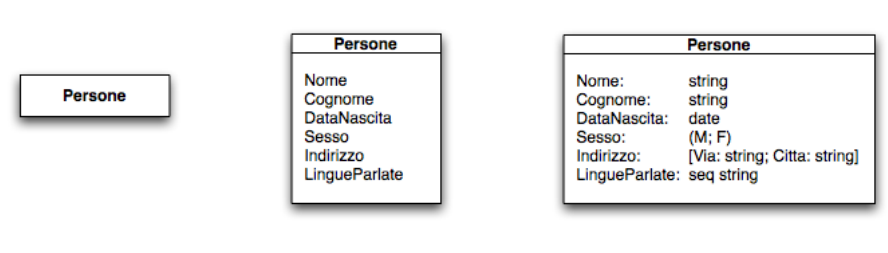
\includegraphics[scale=0.75]{classspec.png}
\end{center}
\paragraph{Tipo oggetto} Il primo passo nella costruzione di un modello consiste nella classificazione delle entità del dominio con la definizione dei tipi degli oggetti che la rappresentano.\\
Un \textbf{tipo oggetto definisce l'insieme dei messaggi} (\textbf{interfaccia}) \textbf{a cui può rispondere un insieme di possibili oggetti}. I nomi dei messaggi sono detti anche attributi degli oggetti.\\
Nei diagrammi ER i tipi oggetti non si rappresentano, perché l'attenzione è sulle collezioni e sulle associazioni. Tuttavia, la rappresentazione grafica di una collezione indica anche gli attributi del tipo oggetto associato.
\paragraph{Associazioni} Un'\textbf{istanza di associazione} è un \textbf{fatto che correla due o più entità}, stabilendo un legame  logico fra loro. Ad esempio, l'utente Tizio ha in prestito una copia della Divina Commedia.\\
Un'associazione \texttt{R(X, Y)} fra due collezioni di entità \texttt{X} e \texttt{Y} è un \textbf{insieme di istanze di associazione} tra elementi di \texttt{X} e di \texttt{Y} che \textbf{varia in generale nel tempo}.\\
Il prodotto cartesiano \texttt{X $\times$ Y} è il dominio dell'associazione.\\
Un esempio:
\begin{center}
	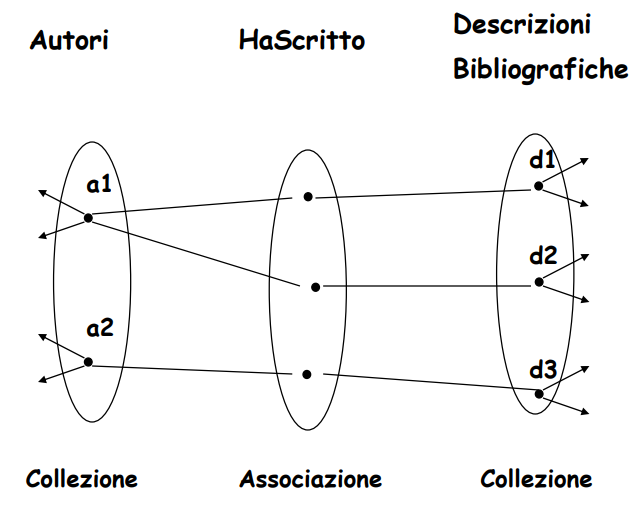
\includegraphics[scale=0.6]{associazioni.png}
\end{center}
\pagebreak
Un associazione è \textbf{caratterizzata da due proprietà strutturali}: \textbf{molteplicità} e \textbf{totalità}.
\subparagraph{Vincolo di univocità} Un'associazione \texttt{R(X, Y)} è \textbf{univoca rispetto a \texttt{X}} se $\forall$\texttt{x} $\in$ \texttt{X} $\exists$ al più un elemento di \texttt{Y} associato ad \texttt{x}.\\
Se non vale questo vincolo, l'associazione è \textbf{multivalore rispetto ad \texttt{X}}.\\\\
\textbf{Cardinalità} dell'associazione:
\begin{list}{}{}
	\item \texttt{R(X, Y)} è \texttt{1:N} se è multivalore su \texttt{X} ed univoca su \texttt{Y}
	\item \texttt{R(X, Y)} è \texttt{N:1} se è univoca su \texttt{X} e multivalore su \texttt{Y}
	\item \texttt{R(X, Y)} è \texttt{N:M} se è multivalore su \texttt{X} e multivalore  su \texttt{Y}
	\item \texttt{R(X, Y)} è \texttt{1:1} se è univoca su \texttt{X} ed univoca su \texttt{Y}
\end{list}
Qualche esempio:
\begin{list}{}{}
	\item \texttt{Frequenta(Studenti, Corsi)} ha cardinalità \texttt{N:M}
	\item \texttt{Insegna(Professori, Corsi)} ha cardinalità \texttt{1:N}
	\item \texttt{SuperatoDa(Esami, Studenti)} ha cardinalità \texttt{N:1}
	\item \texttt{Dirige(Professori, Dipartimenti)} ha cardinalità \texttt{1:1}
\end{list}
\subparagraph{Vincolo di totalità} Un associazione \texttt{R(X, Y)} è \textbf{totale} (o surgettiva) su \texttt{X} se $\forall$ \texttt{x} $\in$ \texttt{X} $\exists$ almeno un elemento di \texttt{Y} associato ad \texttt{x}.\\
Se non vale questo vincolo, l'associazione è \textbf{parziale rispetto a \texttt{X}}.\\
Ad esempio, \texttt{Insegna(Professori, Corsi)} è totale su \texttt{Corsi} perché non può esistere un corso senza il corrispondente docente.
\paragraph{Rappresentazione} Un'associazione si rappresenta con una linea che collega le classi che rappresentano le due collezioni. La linea è etichettata con il nome dell'associazione, di solito scelto utilizzando un predicato.\\
L'univocità dell'associazione rispetto ad una classe si rappresenta disegnando una freccia singola sulla linea che esce dalla classe ed entra nella destinazione. L'assenza di tale vincolo è indicata da una freccia doppia.\\
Similmente, la parzialità è rappresentata da un taglio vicino alla freccia, mentre la totalità è rappresentata dall'assenza del taglio.
\begin{center}
	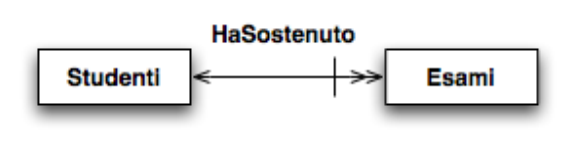
\includegraphics[scale=0.5]{assocesemp.png}\\
	Ogni esame riguarda uno ed un solo studente\\
	Parzialità e assenza di univocità sugli esami\\
	superati da uno studente.\\
	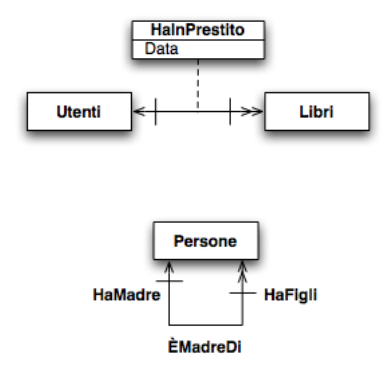
\includegraphics[scale=0.65]{assocesemp2.png}\\
	Possono avere proprietà ed essere ricorsive.
\end{center}
\pagebreak
\subsection{Sottoclassi}
\begin{center}
	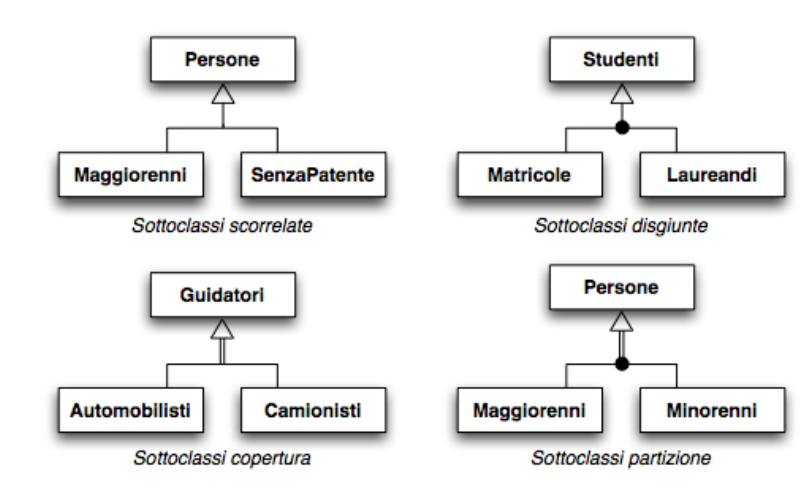
\includegraphics[scale=0.5]{sottoclassi.png}
\end{center}
\paragraph{Vincoli}
\begin{list}{}{}
	\item \textbf{Vincolo intensionale}: C sottoclasse di C' $\Rightarrow$ tipo degli elementi di C è sottotipo del tipo degli elementi di C'
	\item \textbf{Vincolo estensionale}: C sottoclasse di C' $\Rightarrow$ gli elementi di C sono un sottoinsieme degli elementi di C'
	\item \textbf{Disgiunzione}: ogni coppia di sottoclassi è disgiunta, priva di elementi comuni (pallino nero) \textbf{sottoclassi disgiunte})
	\item \textbf{Copertura}: l'unione degli elementi delle sottoclassi coincide con l'insieme degli elementi della superclasse (freccia con doppia asta) (\textbf{sottoclassi copertura})
\end{list}
\subsection{Un esempio elaborato}
\begin{center}
	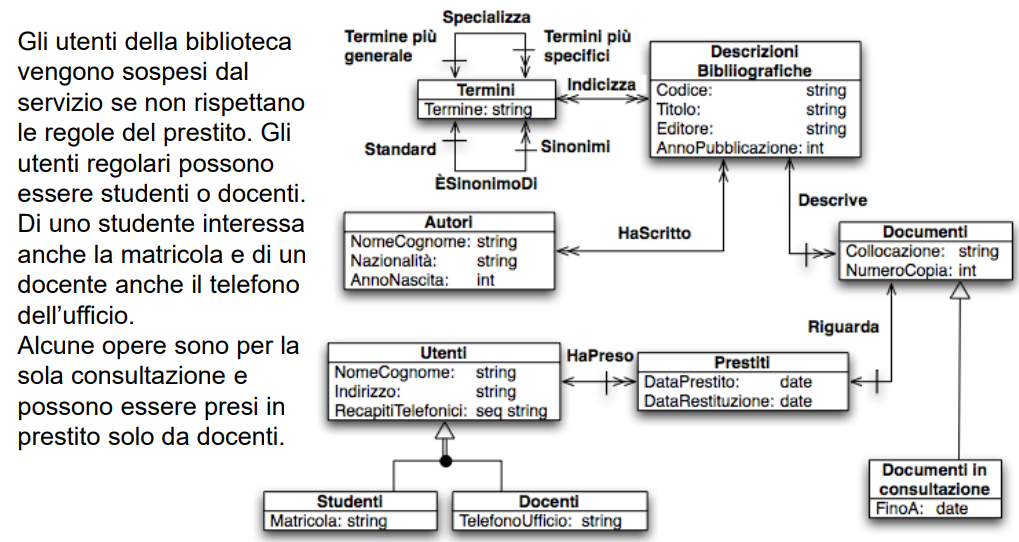
\includegraphics[scale=0.65]{esempioelaborato.png}
\end{center}
\pagebreak
\subsection{Conoscenza astratta}
La conoscenza astratta riguarda i \textbf{fatti generali che descrivono}
\begin{list}{}{}
	\item la \textbf{struttura della conoscenza concreta}, come collezioni, tipi entità, associazioni\ldots
	\item le \textbf{restrizioni sui valori} possibili della conoscenza concreta e sui modi in cui essi possono evolvere nel tempo (\textbf{vincoli d'integrità}, statici e dinamici)
	\item le \textbf{regole per derivare fatti nuovi} da altri noti
\end{list}
\paragraph{Vincoli} Possono essere descritti in \textbf{modo dichiarativo} (da preferire), con formule di calcolo dei predicati, oppure mediante controlli da eseguire nelle operazioni.
\begin{center}
	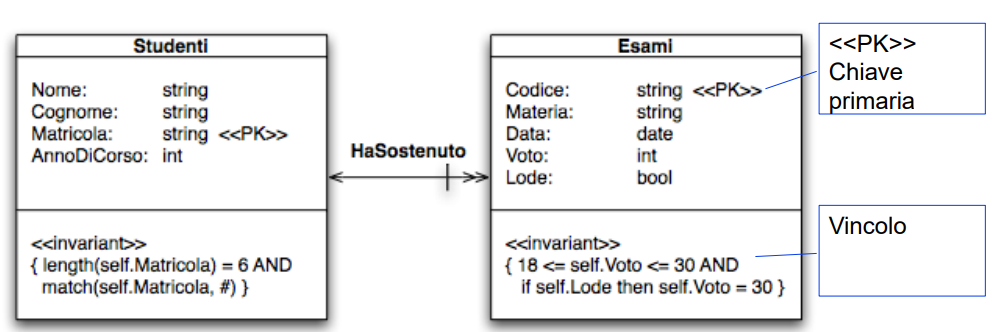
\includegraphics[scale=0.6]{vincoli.png}
\end{center}
\section{Costruzione}
\begin{enumerate}
	\item Analisi dei requisiti $\rightarrow$ specifica dei requisiti, schemi di settore
	\item Progettazione
	\begin{list}{-}{}
		\item Progettazione \textbf{concettuale} ($\rightarrow$ schema concettuale), \textbf{logica} ($\rightarrow$ schema logico), \textbf{fisica} ($\rightarrow$ schema fisico) dei dati
		\item Progettazione delle applicazioni
	\end{list}
	\item Realizzazione
\end{enumerate}
Spesso consideriamo l'analisi dei requisiti come parte della progettazione.
\subsection{Analisi dei requisiti}
\textbf{Analizza il sistema} esistente e \textbf{raccoglie requisiti informali}. Dopodiché \textbf{elimina le ambiguità} e la disuniformità, \textbf{raggruppando frasi relative a diverse categorie} di dati, vincoli e operazioni.\\
Costruisce un \textbf{glossario}, \textbf{disegna lo schema} di settore, \textbf{specifica le operazioni} e \textbf{verifica la coerenza tra operazioni e dati}.
\paragraph{Documentazione descrittiva} In generale, il linguaggio naturale è pieno di ambiguità e fraintendimenti, che bisogna evitare per quanto possibile. Come prima approssimazione si può seguire queste regole:
\begin{list}{}{}
	\item Studiare e comprendere il sistema informativo ed i bisogni informativi di tutti i settori dell'organizzazione
	\item \textbf{Scegliere} il corretto \textbf{livello di astrazione}
	\item \textbf{Standardizzare la scrittura delle frasi}
	\item \textbf{Suddividere le frasi} articolate
	\item \textbf{Separare} le frasi sui \textbf{dati} da quelle sulle \textbf{funzioni}
\end{list}
\paragraph{Organizzare i concetti e i termini} Regole generali
\begin{list}{}{}
	\item Eliminare le ambiguità, le imprecisioni e la disuniformità: individuare omonimi e sinonimi e unificare i termini
	\item Riorganizzare le frasi per \textbf{concetti}, ovvero ottenendo diverse categorie di dati, vincoli e operazioni
	\item Costruire un \textbf{glossario} dei termini
	\item Disegnare lo schema
	\item Specificare le operazioni
	\item Verificare la coerenza fra le operazioni e i dati
\end{list}
\section{Modello Relazionale}
\paragraph{Origini} Proposto da E. F. Codd nel 1970 per favorire l'indipendenza dei dati, disponibile in DBMS reali dal 1981 (non è facile implementare l'indipendenza con efficienza e affidabilità). Si basa sul \textbf{concetto matematico di relazione} con una variante, naturalmente rappresentata come \textbf{tabella}.
\subsection{Relazione matematica}
\paragraph{Dalla teoria degli insiemi} Dati $n$ insiemi anche non distinti $D_1,\ldots,D_n$.\\
Il \textbf{prodotto cartesiano} $D_1\times\ldots\times D_n$ è l'insieme di tutte le $n$-uple $(d_1,\ldots,d_n)$ tali che $d_1\in D_1, \ldots, d_n \in D_n$\\\\
Una \textbf{relazione matematica} su $D_1,\ldots, D_n$ \textbf{è un sottoinsieme di $D_1\times\ldots\times D_n$}, con $D_1,\ldots, D_n$ detti \textbf{domini della relazione}.
\paragraph{Un esempio} Dati $D_1 = \{a, b\}$ e $D_2 = \{x, y, z\}$.\\
Il prodotto cartesiano è l'insieme $D_1\times D_2 = \{(a,x),(a,y),(a,z),(b,x),(b,y),(b,z)\}$\\
Una relazione $r$ potrebbe essere $r\subset D_1\times D_2 = \{(a,x),(a,z),(b,y)\}$
\paragraph{Proprietà} Una relazione matematica è un insieme di $n$-uple ordinate $(d_1,\ldots,d_n)$ tali che $d_1\in D_1, \ldots, d_n \in D_n$.\\
Osservazioni: una relazione è un insieme, quindi
\begin{list}{}{}
	\item non c'è ordinamento fra le $n$-uple
	\item le $n$-uple sono distinte
	\item \textbf{ciascuna $n$-upla è ordinata}, cioè l'$i$-esimo valore proviene dall'$i$-esimo dominio
\end{list}
\paragraph{Tabelle} Una tabella rappresenta una relazione se:
\begin{list}{}{}
	\item I valori di ogni colonna sono fra loro omogenei
	\item Le righe sono diverse fra loro
	\item Le intestazioni delle colonne sono diverse fra loro
\end{list}
In una tabella che rappresenta una relazione \textbf{l'ordinamento} tra le righe e l'ordinamento tra le colonne \textbf{è irrilevante}
\pagebreak
\subsection{Valori}
\paragraph{Il modello relazionale è basato sui valori} Ciò significa che i riferimenti fra dati in relazioni diverse sono rappresentati per mezzo di valori dei domini che compaiono nelle $n$-uple.
\begin{center}
	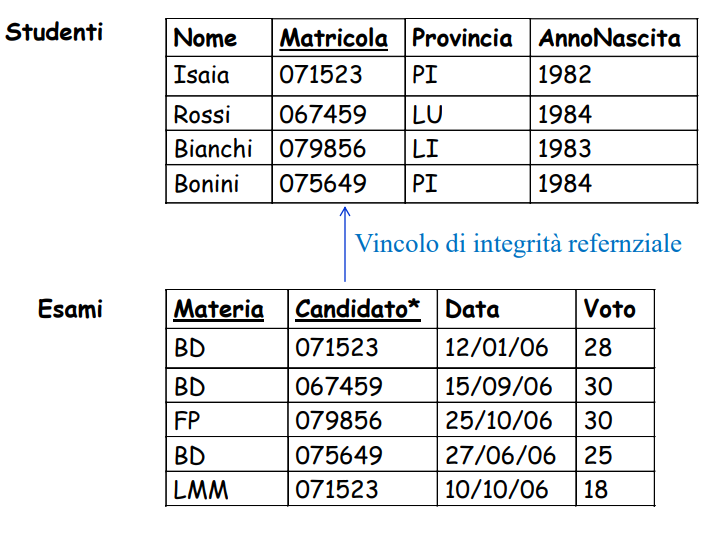
\includegraphics[scale=0.5]{integ.png}
\end{center}
\paragraph{Vantaggi}
\begin{list}{}{}
	\item \textbf{Indipendenza delle strutture fisiche} che possono cambiare dinamicamente, che potremmo avere anche con puntatori di alto livello. La rappresentazione logica dei dati (che è costituita dai soli valori) non fa riferimento a quella fisica.
	\item Si \textbf{rappresenta solo ciò che è rilevante} dal punto di vista dell'applicazione
	\item I \textbf{dati} sono \textbf{portabili} più facilmente da un sistema all'altro
	\item I \textbf{puntatori} sono \textbf{direzionali}
\end{list}
\subsection{Meccanismi}
\paragraph{Definizione} I meccanismi per definire una base di dati con il modello relazionale sono l'\textbf{ennupla} e la \textbf{relazione}.
\paragraph{Tipo ennupla} Un tipo ennupla T è un insieme finito di coppie $\langle$attributo, tipo elementare$\rangle$\\
Se T è un tipo ennupla, R(T) è lo schema della relazione R, quindi \textbf{lo schema di un DB è l'insieme di schemi di relazione R$_i$(T$_i$)}. Un'\textbf{istanza} di uno schema R(T) è un insieme finito di ennuple di tipo T.
\paragraph{Informazione incompleta} Per rappresentare un'informazione incompleta (es.: l'assenza del secondo nome) \textbf{non bisogna usare elementi del dominio} come lo 0, stringa vuota, "99"\ldots.\\
Questo perché potrebbero non esistere valori "non utilizzati", e se esistono potrebbero diventare significativi. Inoltre, in fase di utilizzo (nei programmi) bisognerebbe tenere conto ogni volta del "significato" di questi valori.\\\\
Il \textbf{valore nullo} denota l'\textbf{assenza di un valore del dominio e non è un valore del dominio}.\\
Quindi t[A] per ogni attributo A è un valore del dominio dom(A) oppure è il valore nullo NULL.\\
Si possono (e \textbf{devono}) imporre restrizioni sulla presenza di valori sulli.
\paragraph{Vincoli d'Integrità} Esistono istanze di DB che, nonostante siano sintatticamente corrette, non rappresentano informazioni possibili per l'applicazione e che quindi \textbf{generano informazioni prive di significato}. Ad esempio un voto di 32, o due studenti con la stessa matricola.\\
Uno \textbf{schema relazionale è costituito da un insieme di schemi di relazione e un insieme di vincoli d'integrità} sui possibili valori delle estensioni delle relazioni.\\
Un \textbf{vincolo d'integrità} è una \textbf{proprietà che deve essere soddisfatta dalle istanze che rappresentano informazioni corrette} per l'applicazione.
\pagebreak
\begin{list}{}{}
	\item \textbf{Vincoli Intrarelazionali}: sono vincoli che \textbf{devono essere rispettati dai valori contenuti nella relazione considerata}. Vincoli \textbf{sui valori} (o \textbf{di dominio}), vincoli \textbf{di ennupla}.
	\item \textbf{Vincoli Interrelazionali}: sono vincoli che \textbf{devono essere rispettati da valori contenuti in relazioni diverse}.
\end{list}
\paragraph{Chiave} Informalmente, una \textbf{chiave} è un \textbf{insieme di attributi che identificano le ennuple di una relazione}.\\
Formalmente, \textbf{un insieme K di attributi è \textit{superchiave} per $r$ se $r$ \textit{non} contiene due ennuple distinte $t_1$ e $t_2$ con $t_1[K] = t_2[K]$}.\\
\textbf{K è chiave per $r$ se è superchiave minimale per $r$}, cioè se non contiene altre superchiavi.\\
Un esempio classe è la matricola: è superchiave ed è un solo attributo, quindi è minimale.\\\\
Una relazione non può contenere ennuple distinte ma con valori uguali. Ogni relazione ha \textbf{sicuramente} come superchiave l'insieme di tutti gli attributi su cui è definita, quindi ogni relazione ha (almeno) una chiave.\\
L'esistenza delle chiavi garantisce l'accesso di ciascun dato della base di dati e permettono di correlare i dati in relazioni diverse.\\
Un valore nullo in una chiave non permette di identificare le ennuple o realizzare i riferimenti con altre relazioni. Una \textbf{chiave primaria} è una chiave su cui non sono ammessi valori nulli: si denota sottolineando il nome dell'attributo es. \underline{matricola}.
\paragraph{Integrità referenziale} Le informazioni in relazioni diverse sono correlate attraverso valori comuni. In particolare, \textbf{vengono prese in considerazione i valori delle chiavi primarie}, quindi le \textbf{correlazioni devono essere coerenti}.\\
Un \textbf{vincolo di integrità referenziale} (foreign key) \textbf{fra gli attributi X di una relazione R$_1$ e un'altra relazione R$_2$ impone ai valori su X in R$_1$ di comparire come valori della chiave primaria di R$_2$}.
\section{Trasformazione di schemi}
\paragraph{Progettazione logica} L'obiettivo della progettazione logica è \textbf{tradurre lo schema concettuale in uno schema logico relazionale}, che rappresenti gli stessi dati, \textbf{in maniera corretta ed efficiente}. Questo richiede una ristrutturazione del modello concettuale.
\subsection{Progettazione logica relazionale}
\paragraph{Passaggi} La progettazione di uno schema ad oggetti in uno schema relazionale avviene seguendo questi passaggi:
\begin{enumerate}
	\item rappresentazione delle associazioni 1:1 e 1:N
	\item rappresentazione delle associazioni N:M o non binarie
	\item rappresentazione delle gerarchie d'inclusione
	\item identificazione delle chiavi primarie
	\item rappresentazione degli attributi multivalore
\end{enumerate}
\paragraph{Obiettivo} Rappresentare le \textbf{stesse informazioni}, \textbf{minimizzando la ridondanza} e \textbf{producendo uno schema comprensibile} che faciliti la scrittura e la manutenzione delle applicazioni.
\subsection{Rappresentazione delle associazioni}
\paragraph{Uno a molti} Si rappresentano aggiungendo agli attributi della relazione rispetto a cui l'associazione è univoca la chiave esterna che riferisce l'altra relazione.
\begin{center}
	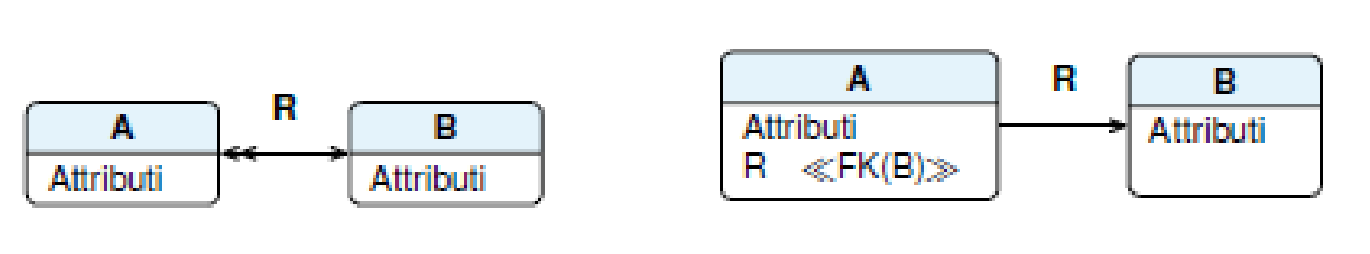
\includegraphics[scale=0.25]{ass1n.png}
\end{center}
\paragraph{Uno a uno} Si rappresentano aggiungendo la chiave esterna ad una qualunque delle due relazioni che riferisce l'altra relazione. Nel caso di un vincolo di totalità, la chiave esterna viene aggiunta alla relazione rispetto cui l'associazione è totale.
\begin{center}
	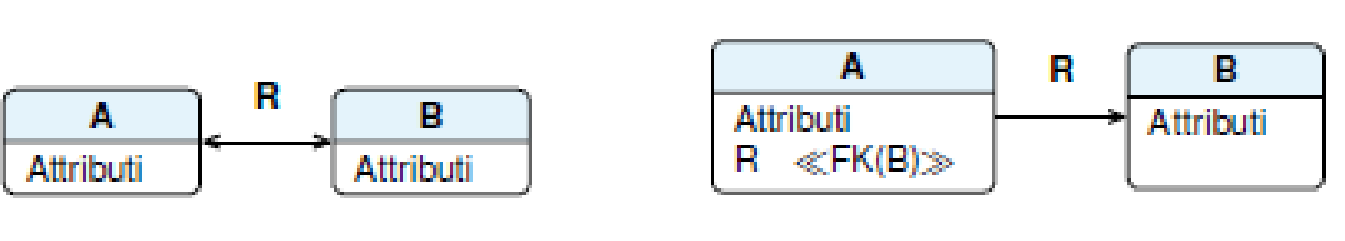
\includegraphics[scale=0.25]{ass11.png}
\end{center}
\paragraph{Molti a molti} Si rappresenta aggiungendo allo schema una nuova relazione contenente due chiavi esterne che riferiscono le due relazioni coinvolte. La chiave primaria di questa relazione è costituita dall'insieme di tutti i suoi attributi.
\begin{center}
	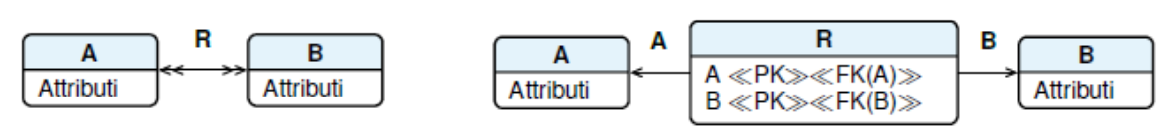
\includegraphics[scale=0.35]{assnn.png}
\end{center}
\subsection{Rappresentazione delle gerarchie fra classi}
Il modello relazionale non può rappresentare direttamente le generalizzazioni. Bisogna eliminare le gerarchie, sostituendole con classi e relazioni:
\begin{list}{}{}
	\item \textbf{Relazione unica}: accorpamento delle figlie della generalizzazione nel genitore\\
	Se $A_0$ è la classe genitore di $A_1$ e $A_2$, allora $A_1$ e $A_2$ vengono eliminate e accorpate ad $A_0$. Ad $A_0$ viene aggiunto un attributo (\textbf{discriminatore}) che indica da quale delle classi figlie deriva una certa istanza, e \textbf{gli attributi di $A_1$ e $A_2$ vengono assorbiti da $A_0$}, assumendo valore nullo sulle istanze provenienti dall'altra classe.
	\begin{center}
		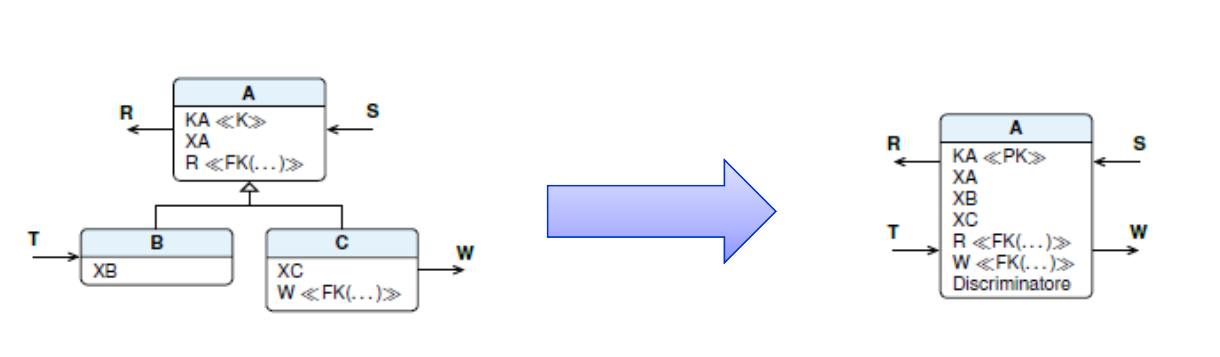
\includegraphics[scale=0.5]{relazunica.png}
	\end{center}
	\item \textbf{Partizionamento orizzontale}: accorpamento del genitore della generalizzazione nelle figlie\\
	La classe genitore $A_0$ viene eliminata e le classi figlie $A_1$ e $A_2$ ereditano le proprietà (attributi, identificatore e relazioni) della classe genitore. Le relazioni della classe genitore vengono sdoppiate, coinvolgendo ciascuna delle figlie.\\
	Divide gli elementi della superclasse in più relazioni diverse, per cui \textbf{non è possibile mantenere un vincolo referenziale verso la superclasse stessa}. Quindi, \textbf{non si usa se nello schema relazionale grafico c'è una freccia che entra nella superclasse} (come la $\leftarrow^S$ nell'esempio sopra, che entra nella superclasse $A$).
	\begin{center}
		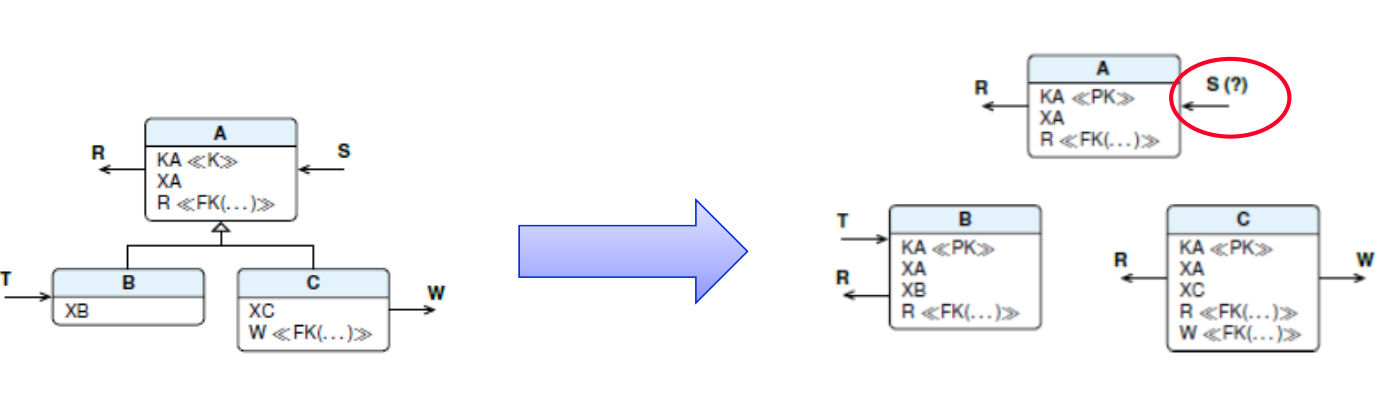
\includegraphics[scale=0.45]{partorizz.png}
	\end{center}
	\item \textbf{Partizionamento verticale}: sostituzione della generalizzazione con relazioni.\\
	La generalizzazione si trasforma in due associazioni uno ad uno che legano rispettivamente la classe progenitore con le classi figlie. In questo caso, \textbf{non c'è un trasferimento di attributi o di associazioni} e le classi figlie $A_1$ e $A_2$ sono identificate esternamente dalla classe genitore $A_0$.\\
	Nello schema ottenuto si aggiungono dei vincoli: ogni occorrenza di $A_0$ non può partecipare contemporaneamente alle due associazioni e se la generalizzazione è totale, deve partecipare almeno una delle due.
	\begin{center}
		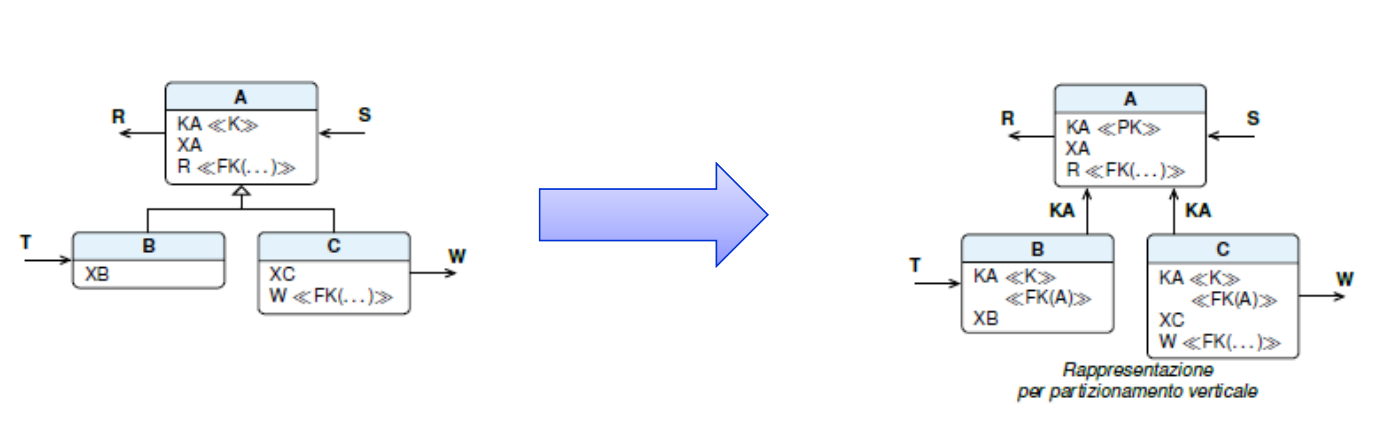
\includegraphics[scale=0.45]{partvert.png}
	\end{center}
\end{list}
\chapter{Algebra Relazionale}
\section{Linguaggi}
\paragraph{Linguaggi per i DB}
\begin{list}{}{}
	\item \textbf{DDL} \textbf{Data Definition Language}, per le \textbf{operazioni sullo schema}.\\
Operazioni di creazione, cancellazione e modifica di schemi di tabelle, creazione viste, creazione indici\ldots
	\item \textbf{DML} \textbf{Data Manipulation Language}, per le \textbf{operazioni sui dati}.\begin{list}{}{}
	\item \textbf{Data Query Language}, per le \textbf{query}, cioè l'\textbf{interrogazione del DB}
	\item \textbf{Aggiornamento dati}, per inserimento, cancellazione e modifica dei dati.
\end{list}
\end{list}
\paragraph{Linguaggi relazionali}
\begin{list}{}{}
	\item \textbf{Algebra relazionale}: insieme di operatori su relazioni che danno come risultato altre relazioni.\\
	Non si usa come linguaggio di interrogazione dei DBMS ma come rappresentazione interna delle interrogazioni.
	\item \textbf{Calcolo relazionale}: linguaggio dichiarativo di tipo logico da cui è stato derivato l'SQL.
\end{list}
\section{Operatori}
\begin{list}{}{}
	\item Unione, intersezione e differenza
	\item Ridenominazione
	\item Selezione
	\item Proiezione
	\item Join (naturale, prodotto cartesiano, theta-join)
\end{list}
Sono \textbf{operatori insiemistici}: \textbf{le relazioni sono insiemi} e i risultati devono essere relazioni a loro volta. L'unione, intersezione e differenza sono applicabili solamente a relazioni definite sugli stessi attributi, cioè \textbf{possono operare solo su tuple uniformi}.
\subsection{Ridenominazione}
\paragraph{Operatore monadico} Un solo argomento, modifica lo schema lasciando inalterata l'istanza dell'operando. Si indica con la lettera $\rho$, esempio: $\rho$ 
\textit{nomecolonna}$\leftarrow$\textit{nuovonome}
\subsection{Proiezione}
\paragraph{Operatore monadico} Produce un risultato che ha \textbf{parte degli attributi} dell'operando e \textbf{contiene ennuple cui contribuiscono tutte le ennuple dell'operando ristrette agli attributi nella lista}. Esempio $\pi_{\textsl{lista attributi}}$(\textit{operando})\\
$\pi_{A_1\ldots A_n}$(\textit{R})\\
Contiene \textbf{al più} tante ennuple quante l'operando, ma può contenerne meno. Se $X$ è superchiave di R, allora $\pi_X$(R) contiene esattamente tante ennuple quante R. Se $X$ non è superchiave, \textbf{potrebbero esistere valori ripetuti su quegli attributi}, che quindi \textbf{vengono rappresentati una sola volta}.
\pagebreak
\subsection{Selezione}
\paragraph{Operatore monadico} Produce un risultato con \textbf{lo stesso schema dell'operando}, \textbf{contiene un sottoinsieme delle ennuple dell'operando} cioè quelle che \textbf{soddisfano una condizione} espressa combinando con i connettivi logici $\wedge$, $\vee$, $\neg$, condizioni atomiche del tipo $A\Theta B$ o $A\Theta c$ dove $\Theta$ è un operatore di confronto, $A$ e $B$ sono attributi su cui l'operatore $\Theta$ abbia senso e $c$ sia una costate compatibile col dominio di $A$.\\
Viene denotata con $\sigma_{\textsl{condizione}}$(\textit{operando}), ad esempio $\sigma_{Stipendio>50\:\wedge\:Filiale='Milano'}$(Impiegati)\\
Per riferirsi ai valori nulli si usano apposite condizioni IS NULL e IS NOT NULL.\\
\begin{center}
$\sigma_{eta>30}$(Persone) $\cup\:\:\sigma_{eta\leq 30}$(Persone) $\cup\:\:\sigma_{eta\:\:IS\:NULL}$(Persone)\\
$=$\\
$\sigma_{eta>30\:\:\vee\:\:eta\leq 30\:\:\vee\:\:eta\:IS NULL}$(Persone)\\
$=$\\
Persone
\end{center}
\begin{center}
	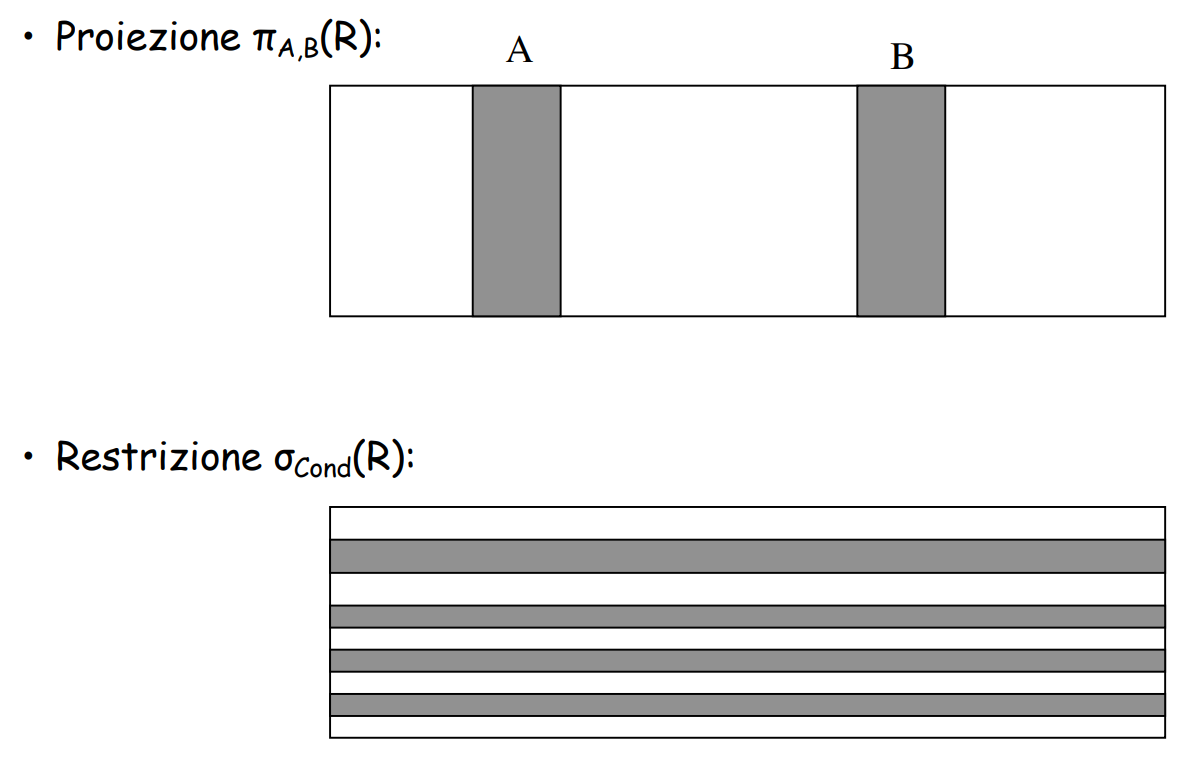
\includegraphics[scale=0.4]{proiezrestriz.png}
\end{center}
\subsection{Join}
\paragraph{Giunzione} Combinando selezione e proiezione possiamo estrarre informazioni da una relazione, ma \textbf{non possiamo correlare informazioni presenti in relazioni diverse}.\\
Il \textbf{join} è l'operatore più interessante dell'algebra relazionale perché consente di correlare i dati in relazioni diverse.
\paragraph{Join naturale} Operatore binario (generalizzabile) che \textbf{correla dati} in relazioni diverse \textbf{sulla base di valori uguali in attributi con lo stesso nome}.\\
Produce un risultato sull'unione degli attributi degli operandi con \textbf{ennuple ottenute combinando le ennuple degli operandi con valori uguali sugli attributi in comune}.\\
Dati $R_1(X_1)$, $R_2(X_2)$, allora $R_1\bowtie R_2$ è una relazione su $X_1\cup X_2$\\
$R_1\bowtie R_2 = \{t$ su $X_1\cup X_2\:|\:\exists t_1\in R_1 \wedge t_2\in R_2$ con $t[X_1] = t_1$ e $t[X_2] = t_2\}$
\subparagraph{Cardinalità} Dati $R_1(A,B)$ e $R_2(B,C)$, il join contiene un numero di ennuple compreso fra 0 e $|R_1|\cdot|R_2|$
$$0 \leq |R_1 \bowtie R_2|\leq |R_1|\cdot|R_2|$$
Se il join è completo, allora contiene un numero di ennuple almeno uguale al massimo tra $|R_1|$ e $|R_2|$. Se il join coinvolge una chiave B di $R_2$, allora $0 \leq |R_1 \bowtie R_2|\leq |R_1|$.\\
Se coinvolge una chiave B di $R_2$ e un vincolo di integrità referenziale tra attributi di $R_1$ e la chiave di $R_2$,\\allora $|R_1 \bowtie R_2| = |R_1|$
\paragraph{Join esterno} Estende con valori nulli le ennuple che verrebbero tagliate fuori da un join interno.\\
Esiste in tre versioni:
\begin{list}{}{}
	\item \textbf{Sinistro} $R \overleftarrow{\bowtie} S$, mantiene tutte le ennuple del primo operando estendendole con valori nulli se necessario.
	\item \textbf{Destro} $R \overrightarrow{\bowtie} S$, idem ma del secondo operando.
	\item \textbf{Completo}, idem ma di entrambi gli operandi.
\end{list}
\paragraph{Prodotto cartesiano} Un join naturale senza attributi in comune: contiene sempre un numero di ennuple pari al prodotto delle cardinalità degli operandi.
\paragraph{Theta-join} Il prodotto cartesiano ha senso solo se seguito da una selezione $\sigma_{condizione}(R_1\bowtie R_2)$, che viene abbreviato con $R_1\bowtie_{condizione}R_2$
\paragraph{Self-join} Non si potrebbe fare una join del tipo Genitore $\bowtie$ Genitore, perché ritornerebbe la stessa tabella Genitore poiché tutti gli attributi coincidono. Torna utile effettuare una ridenominazione del tipo $\rho_{Nonno,Genitore\leftarrow Genitore,Figlio}$(Genitore) per poi effettuare una natural join del risultato con Genitore.
\subsection{Raggruppamento} Con l'operatore $_{\{A_i\}}\gamma_{\{f_i\}}$(R) si effettura il raggruppamento.
\begin{list}{}{}
	\item $A_i$ sono gli \textbf{attributi} di R
	\item $f_i$ sono le \textbf{espressioni} che usano \textbf{funzioni di aggregazione} (min, max, count, sum\ldots)
\end{list}
Il valore del raggruppamento è calcolato come segue:
\begin{list}{}{}
	\item si partizionano le ennuple di R mettendo nello stesso gruppo tutte le ennuple con valori uguali degli $A_i$ (si \textbf{raggruppa per $A_i$})
	\item si \textbf{calcolano le espressioni $f_i$} per ogni gruppo
	\item per ogni gruppo, si \textbf{restituisce una sola ennupla con attributi i valori} degli $A_i$ e delle espressioni $f_i$
\end{list}
\begin{center}
	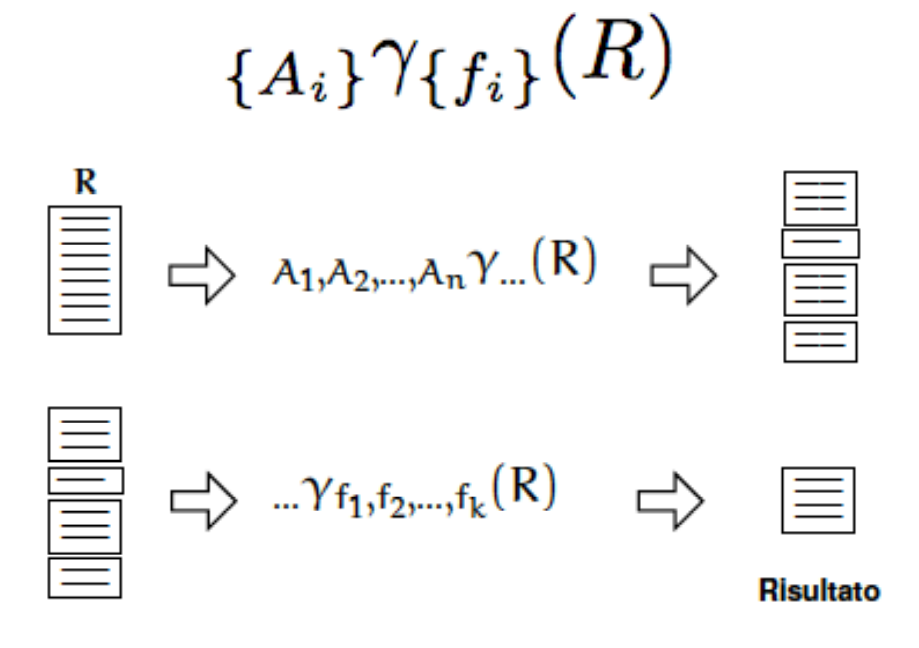
\includegraphics[scale=0.5]{raggrup.png}
\end{center}
\chapter{Interrogazione di una base di dati}
\paragraph{SQL} L'interrogazione di una base di dati è uno degli aspetti più importanti del linguaggio SQL. I comandi di interrogazione, o \textbf{query}, permettono di effettuare una ricerca dei dati presenti nel database che soddisfano particolari condizioni richieste dall'utente.
\begin{lstlisting}
SELECT	s.Nome, e.Data
FROM	Studenti s, Esami e
WHERE	e.Materia = 'BD' AND e.Voto = 30 AND e.Matricola = s.Matricola
\end{lstlisting}
\begin{lstlisting}
SELECT	s.Nome AS Nome, 2020 - s.AnnoNascita AS Eta, 0 AS NumeroEsami
FROM	Studenti s
WHERE	NOT EXISTS(SELECT * FROM Esami e WHERE e.Matricola = s.Matricola)
\end{lstlisting}
\paragraph{Storia} Definito nel 1973, SQL è oggi il linguaggio universale dei sistemi relazionali. Ci sono vari standard (SQL-84, SQL-89\ldots fino a SQL-1999 ANSI/ISO ad oggetti) ed è composto da DDL, DML e \textbf{query language}.
\paragraph{Select From Where} SQL è un \textbf{calcolo su multinsiemi}. Il comando base dell'SQL è:
\begin{lstlisting}
SELECT [DISTINCT] Attributo{, Attributo}
FROM Tabella [Ide]{, Tabella [Ide]}
[WHERE Condizione]
\end{lstlisting}
La semantica è \textbf{prodotto}, \textbf{restrizione}, \textbf{proiezione}. Un attributo A di una tabella "R x" si denota come A, R.A oppure x.A

\begin{lstlisting}
SELECT ListaAttributi
FROM ListaTabelle
[WHERE Condizione]
\end{lstlisting}
La query considera il \textbf{prodotto cartesiano tra le tabelle in \texttt{ListaTabelle}} (\textbf{join}).\\
Fra queste, \textbf{seleziona solo le righe che soddisfano la \texttt{Condizione}} (\textbf{selezione}).\\
Infine, \textbf{valuta le espressioni specificate nella target list \texttt{ListaAttributi}} (\textbf{proiezione}).\\
La SELECT quindi implementa gli operatori di proiezione, selezione e join dell'algebra relazionale.
\subsection{SELECT}
\paragraph{Proiezione} Specifica la target list, cioè corrisponde a scegliere gli attributi della/e tabella/e interessate. Implementa quindi l'operazione di \textbf{proiezione} dell'algebra relazionale.
\subsection{FROM}
\paragraph{Tabelle} Ha lo scopo di scegliere quali sono le tabelle del database da cui vogliamo estrarre le nostre informazioni. Nel caso in cui le tabelle elencate siano due, la FROM insieme alla WHERE implementa il theta-join.
\subsection{WHERE}
\paragraph{Selezione} Serve a scegliere le righe della tabella che soddisfano una certa condizione. In questo modo la clausola WHERE implementa la \textbf{selezione} dell'algebra relazionale.
\paragraph{Condizioni} In SQL sono disponibili una serie di condizioni a seconda del tipo di dato da confrontare, oltre ai IS NULL e IS NOT NULL per i dati mancanti.\\
In particolare, con l'operatore LIKE si possono effettuare ricerche con wildcard: $\%$ per zero o più caratteri, $\_$ per un carattere. Per esempio, \texttt{WHERE Nome LIKE \%a} ricercherà tutti i valori del campo \texttt{Nome} che finiscono per \texttt{a}, oppure \texttt{WHERE Sequenza LIKE \%G\_\_\_G\%} seleziona i valori dove compaiono due \texttt{G} separate da 3 caratteri.\\
Si possono inserire anche dei simboli escape, ad esempio se vogliamo cercare valori in cui compare \texttt{\%} si può scrivere \texttt{WHERE Sconto LIKE \_5\#\% ESCAPE \#}, così da trovare tutti i valori sconto con 5 nelle unità.
\section{Ordinamento e aggregazione}
\paragraph{Ordinamento} Il risultato di una SELECT si può ordinare in base ad un attributo e in maniera crescente o decrescente
\begin{lstlisting}
SELECT ListaAttributi
FROM ListaTabelle
WHERE Condizione
ORDER BY Attributo [ASC/DESC]
\end{lstlisting}
Le righe verranno ordinate in base al campo Attributo in maniera crescente (ASC) o descrescente (DESC). L'ordinamento è quello più naturale sul dominio dell'attributo (numerico, alfabetico\ldots).\\
Si possono anche fare ordinamenti multipli, ad esempio se si vuole ordinare i dati in base ad una certa chiave (attributo) e poi ordinare i dati che coincidono su quella chiave in base ad un'altra chiave (altro attributo).
\begin{lstlisting}
...
ORDER BY Attributo1 [ASC/DESC]{, Attributon [ASC/DESC]}
\end{lstlisting}
Verranno ordinati prima per Attributo1, le righe coincidenti su Attributo1 verranno ordinate per Attributo2\ldots.
\paragraph{Aggregazione} Nella target list possiamo avere anche espressioni che calcolano valori a partire da insiemi di ennuple e che restituiscono una tabella molto particolare, costituita da un \textbf{singolo valore scalare}.\\
Sono 5 gli \textbf{operatori aggregati} previsti da SQL2:
\begin{list}{}{}
	\item \texttt{COUNT()}, conteggio: restituisce il numero di righe della tabella o il numero di valori di un particolare attributo. Con \texttt{(*)} conta tutte le righe selezionate, con \texttt{ALL} conta tutti i valori non nulli delle righe selezionate, \texttt{DISTINCT} conta tutti i valori non nulli distinti delle righe selezionate. Di default è \texttt{ALL}.
	\item \texttt{MIN()}, minimo. L'argomento può essere una funziona aritmetica.
	\item \texttt{MAX()}, massimo. L'argomento può essere una funziona aritmetica.
	\item \texttt{SUM()}, somma. Le specifiche \texttt{ALL} e \texttt{DISTINCT} permettono di sommare tutti i valori non nulli o tutti i valori distinti. Anche qua di default è \texttt{ALL}.
	\item \texttt{AVG()}, media (dei valori non nulli). \texttt{ALL} e \texttt{DISTINCT} per calcolare la media fra tutti i valori o fra quelli distinti, default \texttt{ALL}.
\end{list}
Non è possibile utilizzare, in una stessa SELECT, una proiezione su alcuni attributi della tabella e operatori aggregati sulla stessa tabella. Si possono, invece, fare operazioni aggregate su colonne diverse della stessa tabella.
\paragraph{Raggruppamento} A volta può essere richiesto di calcolare operatori aggregati non per l'intera tabella ma raggruppando le righe i cui valori coincidono su un certo attributo: possiamo scrivere \texttt{GROUP BY Attributo}.\\
Con \texttt{HAVING} si possono applicare condizioni sul valore aggregato per ogni gruppo.\\
Attributo $\rightarrow$ \texttt{WHERE}\\
Operatore aggregato $\rightarrow$ \texttt{HAVING}
\section{Semantica}
La query è innanzitutto eseguita senza operatori aggregati e senza \texttt{GROUP BY}.\\
Quindi il risultato è diviso in sottoinsiemi aventi gli stessi valori per gli attributi elencati in \texttt{GROUP BY}.\\
Quindi l'operatore aggregato è calcolato su ogni sottoinsieme.
\paragraph{Osservazione} Quando si effettua un \textbf{raggruppamento}, questo \textbf{deve essere effettuato su tutti gli elementi della target list che non sono operatori aggregati} (ossia sull'insieme degli attributi puri).\\
Questo perché \textbf{nel risultato deve apparire una riga per ogni gruppo}.
\paragraph{Esempio di query} \texttt{HAVING} può essere usato solo in presenza di un \texttt{GROUP BY} e dopo di esso.
\begin{lstlisting}
SELECT		Citta, Avg(Voto)
FROM		EsamiBD
WHERE		Eta < 21
GROUP BY	Citta
HAVING		AVG(Voto) > 26
\end{lstlisting}
\begin{center}
	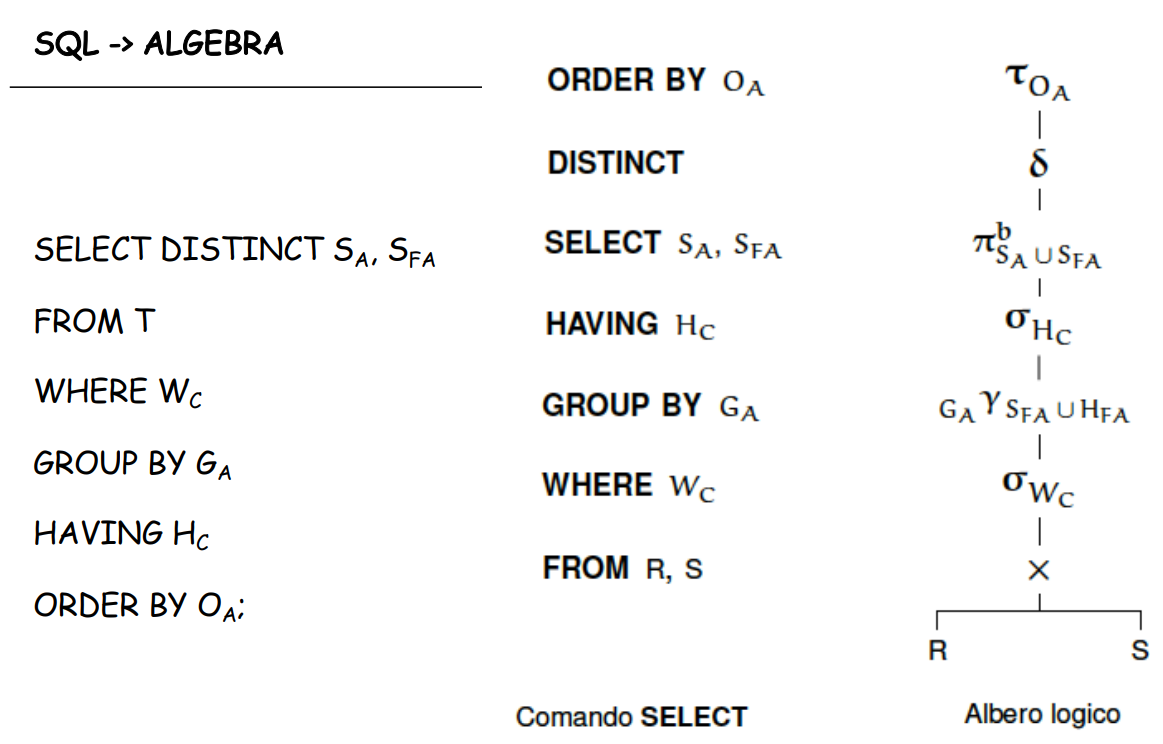
\includegraphics[scale=0.5]{sqlalg.png}
\end{center}
\section{Subquery}
Una \textbf{subquery} un comando SELECT racchiuso tra parantesi tonde ed inserito all'interno di un altro comando SQL (ad esempio un'altra query).\\
Possono essere usate nei seguenti casi:
\begin{list}{}{}
	\item in espressioni di confronto
	\item in espressioni di confronto quantificato
	\item in espressioni IN
	\item in espressioni EXISTS
	\item nel calcolo di espressioni
\end{list}
\paragraph{Tipologie} Ci sono tre tipologie di subquery:
\begin{list}{}{}
	\item \textbf{Subquery Scalare}: comando SELECT che restituisce \textbf{un solo valore}\\
	Es: \texttt{SELECT MAX(Cilindrata) FROM Veicoli}
	\item \textbf{Subquery di Colonna}: comando SELECT che restituisce \textbf{una colonna}\\
	Es: \texttt{SELECT CodCateogira FROM Veicoli}
	\item \textbf{Subquery di Tabella}: comando SELECT che restituisce \textbf{una tabella}\\
	Es: \texttt{SELECT Targa, CodMod, Posti FROM Veicoli}
\end{list}
\pagebreak
\section{Quantificazione}
Tutte le interrogazioni su di un'associazione multivalore vanno quantificate.
\begin{center}
	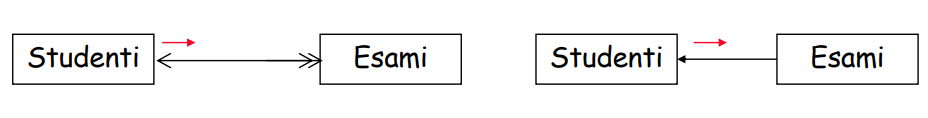
\includegraphics[scale=0.6]{quantific.png}
\end{center}
La query "gli studenti che hanno preso 30" è \textbf{ambigua}.
\begin{list}{}{}
	\item Gli studenti che hanno preso \textbf{sempre} 30: \textbf{universale}
	\item Gli studenti che hanno preso \textbf{almeno un} 30: \textbf{esistenziale}
	\item Gli studenti che \textbf{non} hanno preso \textbf{qualche} 30: \textbf{universale}
	\item Gli studenti che \textbf{non} hanno preso \textbf{sempre} 30: \textbf{esistenziale}
\end{list}
Universale negata = esistenziale\\
Esistenziale negata = universale
\paragraph{ANY, ALL, EXISTS} Le condizioni in SQL permettono il confronto fra un attributo ed il risultato di una subquery che restituisce una colonna od una tabella.
\begin{list}{}{}
	\item Operatore \textbf{scalare} (ANY $|$ ALL) \texttt{SELECT\ldots}\\
	ANY: il predicato è vero se \textbf{almeno uno dei valori restituiti dalla subquery soddisfano la condizione}
	ALL: il predicato è vero se \textbf{tutti i valori restituiti dalla subquery soddisfano la condizione}
	\item Quantificatore \textbf{esistenziale} EXISTS \texttt{SELECT\ldots}\\
	Il predicato è vero se \textbf{la subquery restituisce almeno una tupla}.
\end{list}
\section{Unione, Intersezione, Differenza}
A volte può essere utile poter ottenere un'unica tabella contenente alcuni dei dati contenuti in due tabelle omogenee, ossia con attributi definiti sullo stesso dominio.\\
La SELECT da sola non permette di fare questo tipo di operazioni su tabelle. Esistono per questo dei costrutti espliciti che utilizzano le parole chiave UNION, INTERSECT, EXCEPT (o MINUS).\\
Tali operatori lavorano sulle tabelle come se fossero insiemi di righe, dunque i duplicati vengono eliminati anche dalle proiezioni (a meno di non specificare ALL).\\
Questi operatori vanno in mezzo a due SELECT:
\begin{lstlisting}
SELECT...
(UNION | INTERSECT | EXCEPT) [ALL]
SELECT...
\end{lstlisting}
\paragraph{UNION} Realizza l'operazione di unione definita nell'algebra relazionale. Utilizza come operandi le due tabelle risultanti da comandi SELECT e restituisce una terza tabella che contiene \textbf{tutte le righe della prima e della seconda tabella}.\\
Nel caso in cui dall'unione e dalla proiezione risultassero delle righe duplicate, UNION ne mantiene una sola copia (a meno di aver specificato ALL dopo UNION).\\
\textbf{Mantiene i nomi delle colonne del primo operando}. Quindi, se si vuole ridenominare, è bene ridenominare tutte le colonne che vogliamo.
\paragraph{INTERSECT} Utilizza come operandi due tabelle risultati dai comandi SELECT e restituisce una tabella che contiene \textbf{le righe comuni alle due tabelle iniziali}. Anche qua con ALL mantiene i duplicati, e realizza l'interrsezione dell'algebra relazionale.
\paragraph{EXCEPT} Utilizza come operandi due tabelle ottenute mediante due SELECT, ed ha come risultato una nuova tabella che contiene \textbf{tutte le righe della prima che non si trovano nella seconda}. Realizza la differenza dell'algebra relazionale, ed anche qua si possono mantenere i duplicati utilizzando ALL.
\chapter{Modifica di una base di dati}
\section{Modifica dei dati}
\paragraph{Data Manipulation Language} Introduciamo ora il DML, ossia il linguaggio SQL che serve per \textbf{inserire, modificare e cancellare i dati} del database ma anche per \textbf{interrogare il database} per estrarne i dati.\\
Inizieremo descrivendo le istruzioni che servono a inserire, cancellare e modificare i dati, per poi introdurre le istruzioni per estrarre dal database le informazioni che ci interessano.
\paragraph{INSERT} Per inserire un nuovo dato in una tabella si usa INSERT INTO\ldots VALUES
\begin{lstlisting}
INSERT INTO Tabella [(ListaAttributi)] (VALUES (ListaValori) | Subquery)
\end{lstlisting}
\paragraph{Update} Si possono aggiornare alcuni dati con UPDATE
\begin{lstlisting}
UPDATE Tabella SET Attributo = Expr{, Attributo = Expr} WHERE Condizione
\end{lstlisting}
\paragraph{DELETE} Per cancellare righe dalle tabelle si usa la DELETE
\begin{lstlisting}
DELETE FROM Tabella [WHERE Condizione]
\end{lstlisting}
Per eliminare un elemento bisogna individuare quale, stabilito con la clausola WHERE con la condizione che individua l'elemento (o gli elementi) da eliminare.\\
Un particolare elemento può essere individuato dal suo valore nella chiave primaria.
\section{Definizione degli oggetti}
\paragraph{Data Definition Language} Introduciamo il DDL, cioè il linguaggio SQL che consiste nell'\textbf{insieme delle istruzioni che permettono la creazione, modifica e cancellazione delle tabelle, dei domini e degli altri oggetti del database} al fine di \textbf{definire il suo schema logico}.
\paragraph{Definizione delle tabelle} Le tabelle vengono definite in SQL con l'istruzione \textbf{CREATE TABLE}. Questa istruzione \textbf{definisce uno schema di relazione}, ne \textbf{specifica attributi, domini e vincoli} e ne crea un'istanza vuota.
\begin{lstlisting}
CREATE TABLE NomeTabella
	(NomeColonna1 TipoColonna1 ClausolaDefault1 VincoloColonna1,
	 NomeColonna2 TipoColonna2 ClausolaDefault2 VincoloColonna2,
	 ...
	 NomeColonnak TipoColonnak ClausolaDefaultk VincoloColonnak,
	 VincoliDiTabella
	)
\end{lstlisting}
CREATE TABLE è seguito dal nome della tabella e dalla \textbf{lista delle colonne} (attributi), di cui vengono specificate le caratteristiche. Alla fine si possono anche specificare eventuali vincoli di tabella, di cui parleremo.\\
La CREATE TABLE definisce uno schema di relazione e ne crea un'istanza vuota specificando attributi, domini e vincoli. Una volta create, la tabella è \textbf{pronta} per l'inserimento dei dati (che dovranno soddisfare i vincoli imposti).\\
Lo schema di una tabella, dopo che è stata creata, può essere visualizzato con \textbf{DESCRIBE NomeTabella}.
\pagebreak
\paragraph{Un linguaggio per tanti usi} SQL non è solo un query language, ma anche un linguaggio
\begin{list}{}{}
	\item per la definizione di DB (DDL)
	\begin{lstlisting}
	CREATE SCHEMA Nome AUTHORIZATION Utente
	CREATE TABLE
	CREATE INDEX
	CREATE PROCEDURE
	CREATE TRIGGER
	\end{lstlisting}
	\item per stabilire controlli sull'uso dei dati
	\begin{lstlisting}
	GRANT
	\end{lstlisting}
	\item per la modifica dei dati
\end{list}
\subsection{Tipi}
\paragraph{Tipi} I tipi più comuni per i valori sono:
\begin{list}{}{}
	\item \textbf{CHAR(n)} per stringhe di caratteri di lunghezza fissa $n$
	\item \textbf{VARCHAR(n)} per stringhe di caratteri di lunghezza variabile fino ad un massimo di $n$
	\item \textbf{INTEGER} per interi con la dimensione uguale alla parola di memoria standard dell'elaboratore
	\item \textbf{REAL} per numeri reali con dimensione uguale alla parola di memoria standard dell'elaboratore
	\item \textbf{NUMBER(p,s)} per numeri con $p$ cifre di cui $s$ decimali
	\item \textbf{FLOAT(p)} per numeri binari in virgola mobile con almeno $p$ cifre significative
	\item \textbf{DATE} per valori che rappresentano istanti nel tempo (in alcuni sistemi come Oracle) oppure solo date (con un altro tipo \textbf{TIME} per indicare l'orario)
\end{list}
\paragraph{Un esempio} 
\begin{lstlisting}
CREATE TABLE Impiegati
	(Codice CHAR(8) NOT NULL,
	 Nome CHAR(20),
	 AnnoNascita INTEGER CHECK (AnnoNascita < 2000),
	 Qualifica CHAR(20) DEFAULT 'Impiegato',
	 Supervisore CHAR(8),
	 PRIMARY KEY pk_impiegato (Codice),
	 FOREIGN KEY fk_Impiegati (Supervisore) REFERENCES Impiegati
	)
	
CREATE TABLE FamiliariACarico
	(Nome CHAR(20),
	 AnnoNascita INTEGER,
	 GradoParentela CHAR(10),
	 CapoFamiglia CHAR(8)
	 FOREIGN KEY fk_FamiliariACarico (CapoFamiglia) REFERENCES Impiegati
	)
\end{lstlisting}
\paragraph{Eliminare e modificare} Ciò che viene creato con ALTER TABLE può essere eliminato con \textbf{DROP} o modificato con \textbf{ALTER}. Con \textbf{ALTER TABLE} nello standard SQL è possibile
\begin{list}{}{}
	\item Aggiungere una colonna \textbf{ADD COLUMN}
	\item Rimuovere una colonna \textbf{DROP COLUMN}
	\item Modificare una colonna \textbf{MODIFY}
	\item Aggiungere l'assegnazione di valori di default \textbf{SET DEFAULT} o eliminarli \textbf{DROP DEFAULT}
	\item Aggiungere vincoli di tabella \textbf{ADD CONSTRAINT} o eliminarli \textbf{DROP CONSTRAINT}
	\item Altre opzioni specifica dei linguaggi.
\end{list}
\end{document}